\section{Proposal}
\label{proposal}

\subsection{Analysis of Web Service documentation sources}
\label{subsec:analysis-ws-doc}
As evidenced in the study by Maleshkova et al. \cite{Maleshkova:2010}, web service documentation is often limited by the content that API developers provide on their websites. SOAP services are a special case, whose main descriptor is a WSDL document, which defines an abstract service interface (information regarding operations, messages and types) and concrete details about transport and location of the service. Following subsections deal with the description of mechanisms for extraction of technical information regarding service functionality, from various documentation sources: WSDL descriptors for SOAP services, and HTML pages for XML-RPC and REST services.

\subsubsection{SOAP Services}
\label{subsub:soap}
WSDL is an XML standard format for Web service description [32]. A WSDL document describes service interface abstractly and provides concrete technical details about service operation. This may be visualized in figure \ref{wsdl-Structure}, which shows the structure of a WSDL descriptor.

\begin{figure}
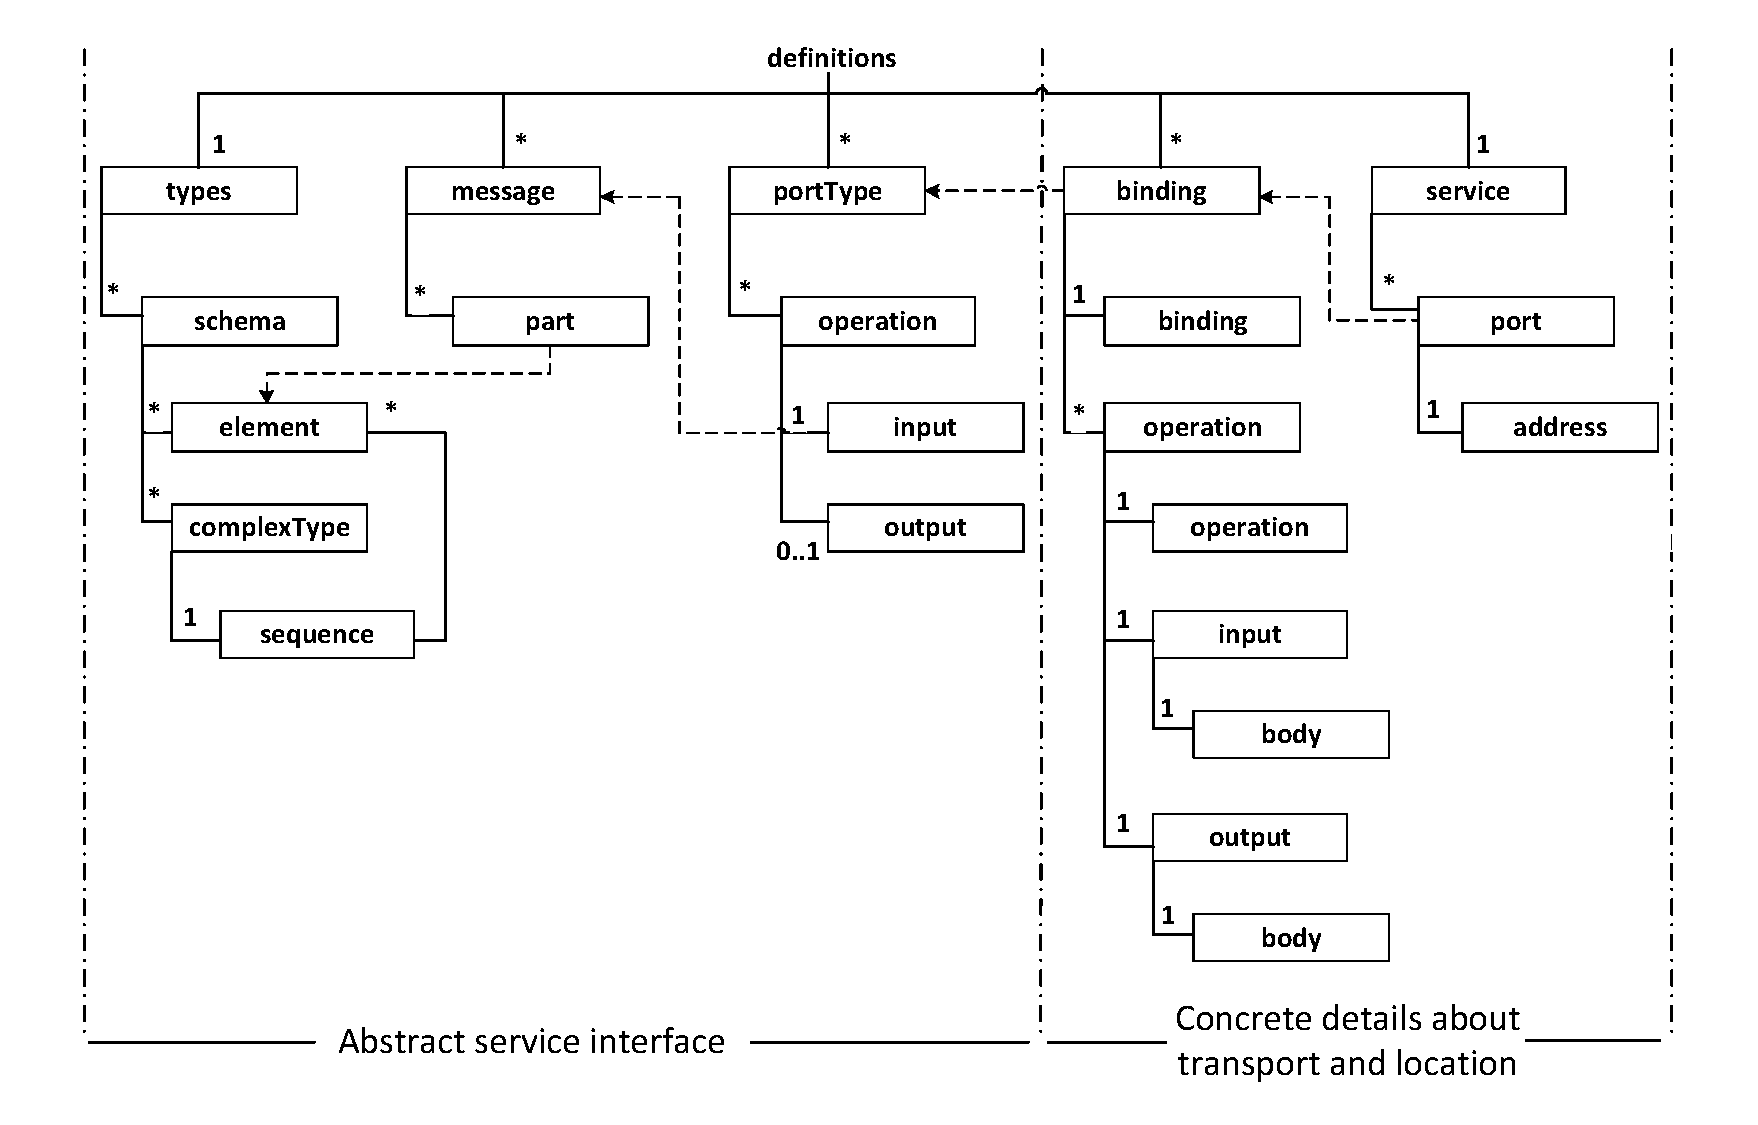
\includegraphics[scale=0.40]{images/wsdl-structure-en}

\caption{Structure of WSDL descriptor.}
\label{wsdl-Structure}
\end{figure}

The diagram of figure \ref{wsdl-Structure}, shows the separation between service’s abstract description and concrete details. The later refer to element that specify service endpoints, and communication and transport protocols used for message exchange. These concrete details are required for service invocation, however they provide little information about service functionality, this is why descriptor analysis focuses on the components of the abstract description of the service interface, namely:

\begin{itemize}
 \item \textit{Types (schema, element, complexElement, sequence)}: define the data types composing the messages exchanged in service invocation.
 \item \textit{Message} : represents an abstract definition of data transmitted when invoking a particular service operation.
 \item \textit{PortType}: it is defined as a grouping of abstract service operations along with their associated messages.
 \item \textit{Operation}: abstracts service functional units. This descriptor element is associated with a set of input/output messages.
\end{itemize}

Additionally, WSDL allows natural language description for some of the service interface elements, including: service, binding, portType, operation, message and types. Such a description is provided by service developers and is enclosed within a special tag called documentation. As argued by Falleri in [8], typically there is some redundancy in the information contained in certain elements of service interface. Thus, for instance, terms defining ports, bindings and portTypes are frequently the same used for describing the service element; likewise terms defining input/output messages, are slight variations of the term specifying their associated operation. In consequence, it was decided that information extraction from service descriptor only takes the content of service, operation and types elements into account, including their natural language descriptions (when available). This way, it is possible to obtain a simplified model of the information the service interface contains, considering the three 
mentioned elements. This model is shown in figure \ref{wsdl-Simplified}.

\begin{figure}
\center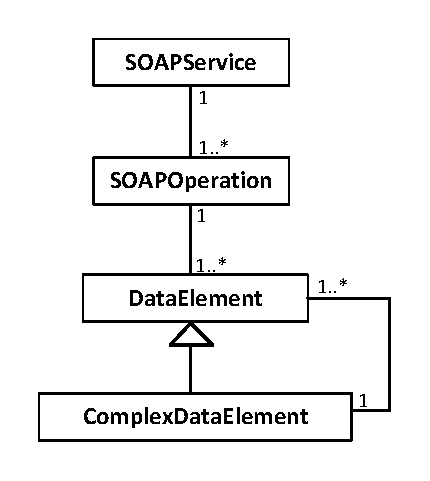
\includegraphics[scale=0.6]{images/wsdl-simplified}

\caption{Simple model for describing SOAP Services.}
\label{wsdl-Simplified}

\end{figure}

In the model above, \emph{DataElement} and \emph{ComplexDataElement} elements represent \emph{simple }and\emph{ complex types} (\emph{types})
respectively, which compose the message exchanged when invoking a service operation. Typically the terms used in defining such elements of the WSDL descriptor follow naming conventions commonly adopted by programmer, e.g. using \texttt{CamelCase} compound words for identifying operations, types and services. Similarly, sometimes documentation tags contain HTML encoded data. Therefore it is necessary to get the content into a proper format to enable further processing. This involves the use of text mining techniques such as \emph{tokenization},\emph{POS (Part-of-speech) tagging } and \emph{spell checking} whose description is addressed in section \ref{subsub:Service-documentation-cleaning}.

\subsubsection{XML-RPC and REST Services}
\label{subsubsec:rpc-rest}
As it was mentioned at the beginning of section \ref{subsec:analysis-ws-doc}, Web service documentation---except for SOAP services---doesn't meet
any standard format. XML-RPC and REST services, are commonly described by HTML pages, which provide information regarding service functionality and endpoints \footnote{For example: (XML-RPC) ,\href{http://www.benchmarkemail.com/API/Library}{http://www.benchmarkemail.com/API/Library} (REST) \href{https://dev.twitter.com/docs/api/1.1}{https://dev.twitter.com/docs/api/1.1}}. Usually the content of such pages doesn't follow a formal structure, making it difficult to extract relevant information in an automated way. There are some initiatives, including \emph{ProgrammableWeb} and
\emph{APIhub} \footnote{Available at: \href{http://www.apihub.com/}{http://www.apihub.com/}}, which promotes the creation of centralized API directories, where service documentation is uniformly stored, by following a regularstructure. However, a major issue regarding these initiatives is that documentation must be registered manually, so more often than not the information provided either contains errors (typos, broken links) or is outdated.

Given this limitation, it was decided to deal with documentation that developers provide on API websites. This way, we apply on each HTML page an analysis that involves identifying recurring patterns (which depends on the service type, either XML-RPC or REST) and document segmentation for extracting relevant information regarding service functionality. This analysis is supported on the approach of Ly et al. formulated in \cite{Ly:2012}.

\paragraph{Analysis of XML-RPC service documentation}
\label{parag:rpc}
Similar to SOAP services, an XML-RPC service defines a set of operations or procedures that clients can invoke remotely. The documentation of this kind of services, deals with the operations they expose, the arguments they require for their invocation, and usually specifies the service endpoint (URI) and the HTTP method used for communication.

The description of operations within the same XML-RPC service documentation tends to share similar structure and content. Thus, for example, operation identifiers are usually defined by terms in \texttt{CamelCase} notation, composed of a verb and a noun (e. g., \emph{getWeather}). Also, given that this kind of documentation is intended for humans, its content is articulated with recurrent visual clues that help identify operation description blocks within the HTML page: e.g., operation identifiers may be enclosed in \texttt{<h3>} tags and their natural language descriptions\emph{ }in \texttt{<p>} tags. Then, it is possible to use those local patterns present in each of the service documentation pages, for extracting the information blocks regarding service operations. 

Prior to the extraction of operation description blocks, a preprocessing step is required for getting rid of images, scripts, malformed tags and formatting tags (\texttt{<b>}, \texttt{<strong>}, \texttt{<i>}, etc.) from HTML documentation pages.

Then the operation description blocks are extracted, by following the steps below: 

\begin{enumerate}
 \item Extraction of \texttt{CamelCase} terms composed of a verb and a noun (which make up the set of candidate operations identifiers), while keeping track of the HTML tag that encloses them.
 \item Identify the most commonly used tag (\emph{elected tag}) for the operation identifiers found in the first step.
 \item Finally, out of all the operation identifiers found in step \#1, only retain identifiers within \emph{elected tags}. The page is then segmented according to the scope of the tags enclosing each of the chosen operation identifiers.
\end{enumerate}

By following the above procedure, it is possible to identify and extract the textual data from operation description blocks, such as that illustrated in Figure \ref{xml-rpc-op-block}.

\begin{figure}
 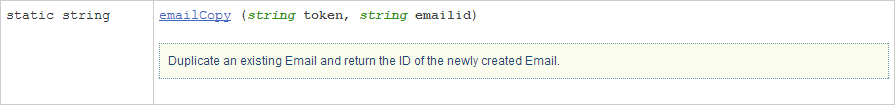
\includegraphics[scale=0.5]{images/xml-rpc-operation-block}

 \caption{Operation description block - XML-RPC service. {\scriptsize Source:
 \protect\href{http://www.benchmarkemail.com/API/Library}{http://www.benchmarkemail.com/API/Library}}}
 \label{xml-rpc-op-block}
\end{figure}

\paragraph{Analysis of REST APIs documentation}
\label{parag:rest}
While nowadays there is a seemingly increasing adoption of the REST architectural style for building web services, actually only a few of them support all the guidelines that REST defines. In terms of the Richardson's maturity model explained in section \ref{sec:motivation_background}, most of the existing REST services are in fact \emph{level one }services\emph{ }(URI supported), while few of them qualify as \emph{level two }(URI \& HTTP supported) and \emph{level three} (RESTFul: URI, HTTP \& Hypermedia supported) services.

Documentation of this kind of services, provided as HTML pages, is focused on the concept of resources and the parameters used for identifying them, which are encoded into URI templates (e.g., \texttt{/\{resource\}/\{property\}/}). In addition, this documentation specifies the allowed HTTP methods
(\texttt{GET, POST, PUT, DELETE}, etcetera) for each of the resources hosted by the service. See for example the documentation available on the website of the twitter API for developers shown in Figure \ref{twitter-rest-api}.

\begin{figure}
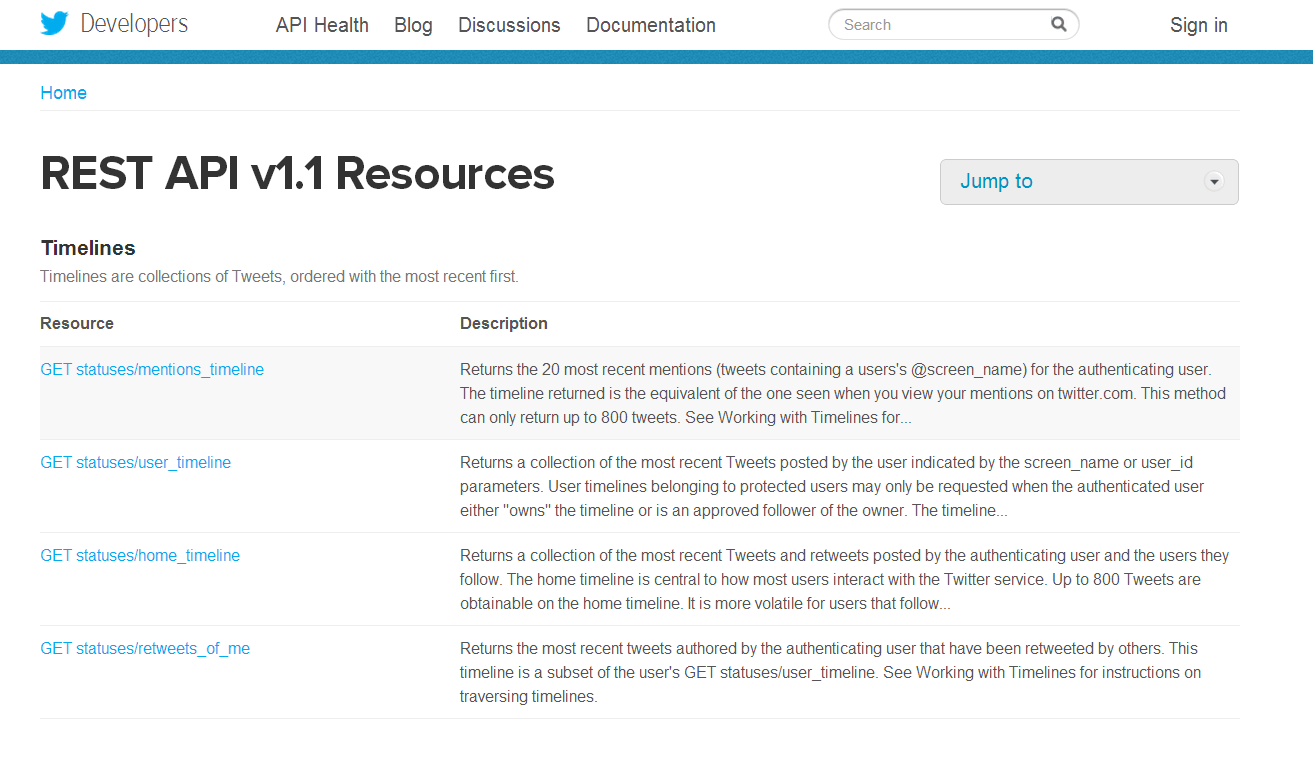
\includegraphics[scale=0.33]{images/twitter-rest-api}

\caption{Documentation of the Twitter REST API.{\scriptsize{} Source: \protect\href{https://dev.twitter.com/docs/api/1.1}{https://dev.twitter.com/docs/api/1.1}}}
\label{twitter-rest-api}

\end{figure}

This way, the analysis of REST services documentation focuses on detection and extraction of resources description blocks, which contain URI templates, HTTP methods and usually a description in natural language. Since REST API developers tend to adopt a recurring pattern for documenting
the service resources, it is possible to perform a segmentation procedure on the HTML content, in order to extract the mentioned description blocks. 

Such a procedure starts from the analysis of the HTML DOM tree to perform the steps listed below:

\begin{enumerate}
 \item Segment the HTML document into blocks containing URIs and HTTP methods. 
 \item Compute the similarity between the blocks found in step \#1, and retain those having the same structure.
 \item Extract the information of each resource, contained within the blocks identified in the previous step: resource URI, supported methods and description in natural language.
\end{enumerate}

For conducting the second step of the previous procedure, the authors of \cite{Ly:2012} rely on the concepts of \emph{entropy} and \emph{node internal structure}. Entropy is a measure that quantifies local patterns present in segments of the HTML document, so that a high entropy suggests
an irregular structure, while a low entropy denotes a substantial similarity. The internal structure of a node from the HTML DOM tree, consists in the concatenation of the tags that make up such node, so for example, given the following page segment \texttt{<div><a><span>link</span></a>\\<p>text</p></div>}, the internal structure of the \texttt{div} node is: \texttt{<div><a><span><p>}.

This way, the entropy measure estimates the similarity between the document segments found in step \#1, which is subsequently used for obtaining the set of resources descriptor blocks included in the service documentation.

\subsubsection{Service documentation pre-processing}
\label{subsub:Service-documentation-cleaning}
Often, the information that developers provide in service descriptors follows naming conventions commonly used in programming languages, in particular they use compound words such as \emph{helloword}, \emph{hello\_world} or \emph{helloWord} for identifying operations, resources and parameters. Also, it might be possible for descriptions in natural language to include content encoded into HTML or XML tags, which are used for formatting the text or providing structure to it. 

A requirement for further analyze the information extracted from service documentation (see end of section \ref{sec:motivation_background}) consists in processing such information and turning it into plain text, which involves splitting compound words and getting rid of HTML or XML tags. To this end it has been decided to use certain text mining techniques, including \emph{tokenization}, \emph{spell checking }and \emph{POS tagging}, whose description is addressed below. 

\paragraph{Tokenization}
\label{parag:tokenization}
This is a procedure that allows breaking a sequence of characters up into its composing tokens. The information extracted from service descriptors is subject to this process to generate the list of terms included within identifiers of operation, resources and types, as well as the text of descriptions in natural language. So, for example the list of tokens contained in the sequence ``\emph{getWeatherByCity}'' is: \{\textquotedblleft{}\emph{get}\textquotedblright{}, \textquotedblleft{}\emph{Weather}\textquotedblright{} \textquotedblleft{}\emph{By}\textquotedblright{}, \textquotedblleft{}\emph{City}\textquotedblright{}\}. In the previous example, the method for breaking the compound term up relies on detecting transition from lowercase to uppercase along the sequence. However, there are some cases where this procedure is not that straightforward: e.g., the sequence ``\emph{getweatherbycity}'' doesn't use letter case for telling tokens apart. In these special cases a spell checking technique is used, as 
outlined next.


\paragraph{Spell checking}
\label{parag:spell-checking}
It is clear for a human that strings \textquotedblleft{}\emph{homeaddress}\textquotedblright{} and \textquotedblleft{}\emph{home address}\textquotedblright{} contain the same information. However for machines those are two different sequences of characters and there is no trivial way for it to tell that they are equivalent strings. This turns out to be a common problem in Information Retrieval \cite{Airio:2006} known as \emph{compound splitting}. For tackling this compound splitting problem, we use a mechanism based on term look up over a tree-like data structure called \emph{Trie} \cite{Fredkin:1960} which in this particular case encodes the terms from the \emph{words }dictionary \footnote{Example available at: \href{http://www.cs.duke.edu/~ola/ap/linuxwords}{http://www.cs.duke.edu/$\sim$ola/ap/linuxwords}}, included in Unix-like operating systems. This data structure usually supports spell checking and autocomplete software, used in search engines and some other web and mobile applications.

\emph{Trie-based }search is similar to the way we look up words in a dictionary, i.e. by using prefixes. For extracting the terms that make up a compound word an iterative procedure is conducted: (1) It divides the sequence of characters into segments with different length; (2) it look up each of the segments in the Trie. This process continues until all the segments obtained in step \#1 match terms included in the dictionary. Table \ref{trie-example}, shows this procedure applied on the sequence \textquotedblleft{}\emph{homeaddress}\textquotedblright{}.

\begin{table}
\caption{Trie-based compound splitting for \textquotedblleft{}\emph{homeaddress}\textquotedblright{}.}


\center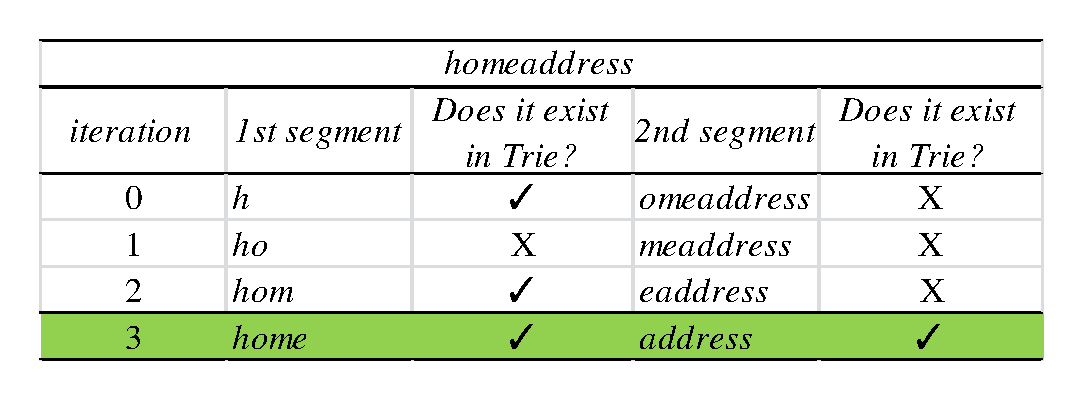
\includegraphics[scale=0.5]{images/example-trie-spellchecking-en}\label{trie-example}
\end{table}



\paragraph{Part-of-speech (POS) tagging}
\label{parag:part-of-speech}
This technique, is used for detecting candidate operations described in the documentation of XML-RPC services. According to the analysis outlined in section \ref{sub:Analysis-of-XML-RPC}, the operations hosted by this kind of services, are frequently identified by \texttt{CamelCase} terms joining at least a verb and a noun (e. g., \emph{getWeather}). POS tagging allows specifying the \emph{lexical category} (verb, noun, pronoun, adverb, etcetera) corresponding to each term in a text or sentence. This way it is possible to filter out the compound words included in XML-RPC service documentation and extracting the set of candidate operations. The POS tagging technique used in our case is the one conceived by Toutanova, outlined in \cite{Toutanova:2003} and developed inside The \emph{Stanford Natural Language Processing Group}.

By applying the techniques explained above on the documentation of Web services, the noise involved in the statistical analysis intended
to identify groups of similar services is reduced. As defined at the end of section \ref{sub:REST-APIs}, this analysis is the second of the key processes that comprise the approach documented herein. The description of this second process is addressed in the section below.

\subsection{Discovering the semantic structure of Web service documentation by applying Probabilistic topic modeling}
\label{subsec:probabilistic-topic-models}

Nowadays the amount of information and resources available on the Web is huge and ever increasing, so that it has exceeded our ability for locating and accessing the resources we need. This way, increasingly sophisticated computational tools are required for organizing, searching and understanding those resources, beyond the traditional information indexing and retrieval approaches. 

In this regard, over the last decade a variety of statistical models known as probabilistic topic models have emerged \cite{Blei:2012} as powerful tools that allow to uncover the hidden thematic structure that runs through a document collection. 

The algorithms developed for applying these models, may be adapted to several types of data collections. There exist for instance, approaches like the one conceived by Chen et al. \cite{Chen:2012} where the authors use topic models for identifying patterns on genomic data, others like \cite{Feng:2010} apply topic models to enable the automatic annotation of images, and others such as \cite{Cha:2012} discuss the application of these models for analyzing the relationship graph from a social network. 

A common application of probabilistic topic model algorithms is the categorization of text collections into groups of documents sharing similar topics, thus enabling a sort of semantic indexing over the items of the collection. The work addressed in this report aims to apply this process of categorization on the textual information extracted from a corpus of Web service description documents, by using a topic model called \emph{online LDA} (\emph{Latent Dirichlet Allocation}) which enable the incremental categorization of a continuous stream of documents. In this particular case, documents contain information regarding each operation or resource from a service collection. In the following sections it is addressed the description of the LDA topic model, and how it was adopted within this research. 

\subsubsection{The Latent Dirichlet Allocation (LDA) topic model}
\label{subsub:The-Latent-Dirichlet}

LDA is one of the most basic and widely adopted probabilistic topic models used for identifying the abstract themes that pervade a documentary corpus \cite{Blei:2003}. In statistical terms, LDA in one of the so-called generative models, which allows sets of observations (i.e. documents) to be explained by hidden or latent variables (topics).

The intuition behind LDA is to assume that documents in the corpus deal with not only one but several topics. This report for example is about \emph{Web services}, \emph{Semantics}, \emph{Topic models}, and \emph{REST}. LDA estimates that documents are generated through the random process outlined below (see Figure \ref{lda-gen-process}): 

\begin{figure}
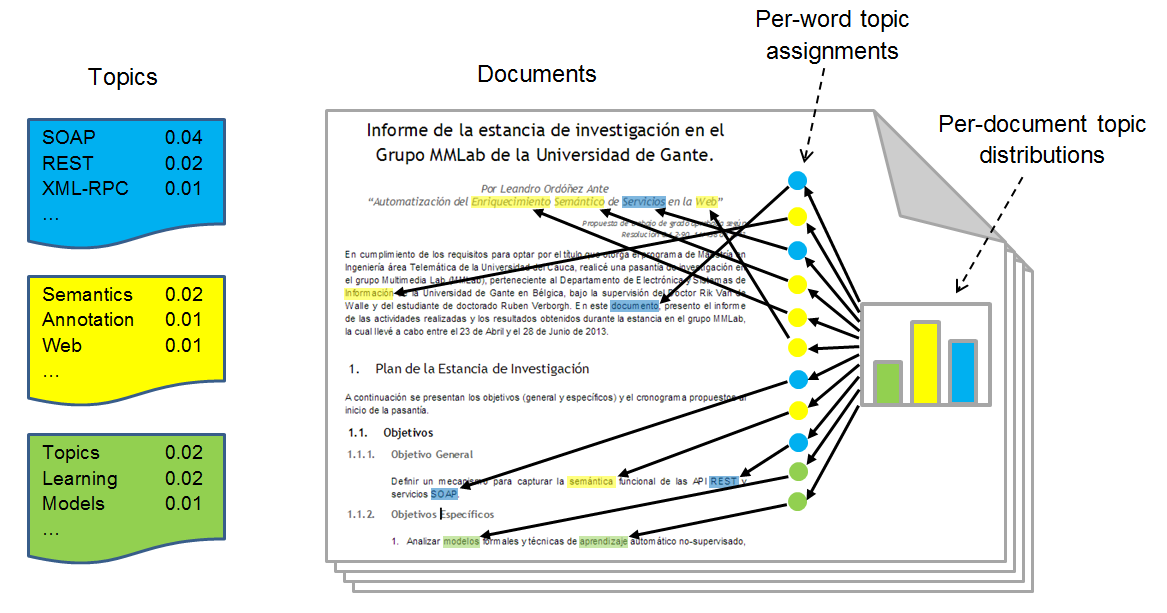
\includegraphics[scale=0.40]{images/lda-gen-model-eng}

\caption{Generative process for LDA. {\scriptsize Adapted from: \cite{Blei:2012}}}
\label{lda-gen-process}
\end{figure}

\begin{itemize}
\item LDA assumes:

\begin{itemize}
\item Each topic is a distribution over the vocabulary composing the whole document collection, excluding stop words such as \textquotedblleft{}\emph{and}\textquotedblright{}, \textquotedblleft{}\emph{or}\textquotedblright{}, \textquotedblleft{}\emph{the}\textquotedblright{}, \textquotedblleft{}\emph{but}\textquotedblright{}, \textquotedblleft{}\emph{of}\textquotedblright{}, etcetera. Thus, for instance, in the ``\emph{Web service}'' topic (the blue one in Figure \ref{lda-gen-process}), terms like ``SOAP'', ``REST'', and ``XML-RPC'' would have high probability of occurrence. 
\item The corpus has a finite number of topics ($K$), which are specified before the documents have been generated. 
\item Word order in each of the documents is not relevant: the documents are modeled as \emph{bags-of-words}. 
\end{itemize}

\item The generative process for each document in the collection is as follows:

\begin{enumerate}
\item Randomly choose a distribution over the topics, as the topic proportions for each document (represented in Figure \ref{lda-gen-process} by the three bar histogram).
\item for each word in the document: 

\begin{enumerate}
\item Randomly choose a topic from the distribution drawn in step \#1. 
\item Randomly choose a word from the topic (distribution over words) drawn in step \#2a. 
\end{enumerate}
\end{enumerate}
\end{itemize}
According to the above process, all the documents in the corpus share the same set of topics, but each one of them has different topic proportions, given by the distribution assigned in step \#1. This way the generative process satisfies the intuition behind LDA by conceiving the documents as a mixture of topics.

Nonetheless, the distributions assumed by this generative process---i.e., topics, per-document topic proportions and per-word topic assignments---are unknown a priori; the only observable variable is the collection of document, as shown in Figure \ref{observable-hidden-vbles-lda}. The aforementioned distributions define hidden variables which could be inferred by ``reversing'' the LDA generative process, allowing to estimate the hidden thematic structure that generates the observed document collection. 

\begin{figure}
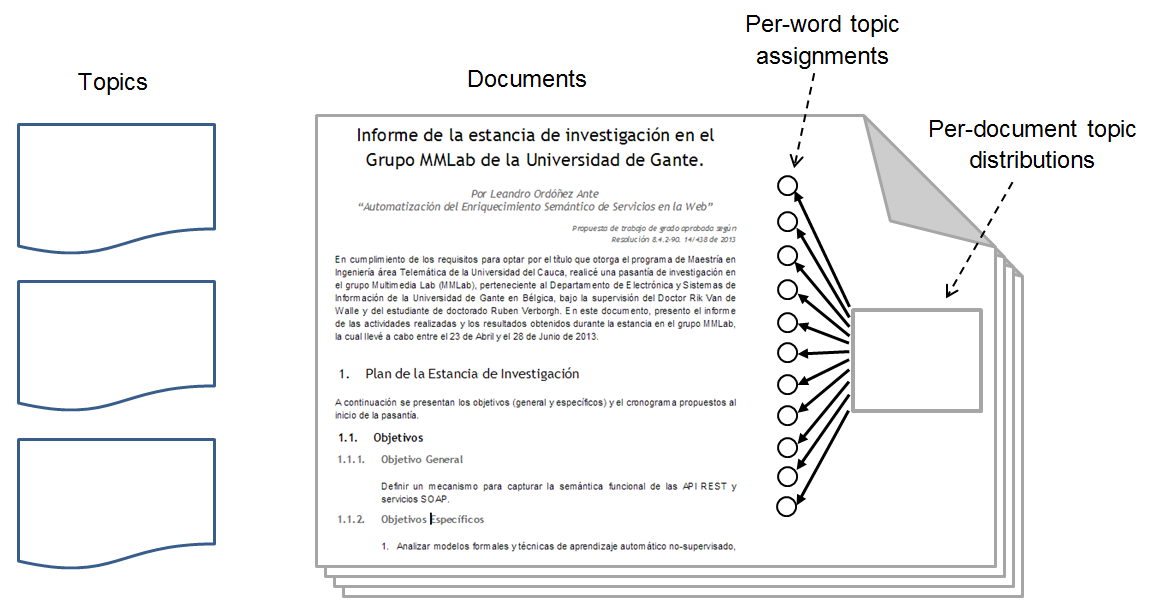
\includegraphics[scale=0.40]{images/lda-gen-model-eng2}

\caption{Observable and hidden variables of the generative process of LDA.
{\scriptsize Adapted from: \cite{Blei:2012}}}
\label{observable-hidden-vbles-lda}
\end{figure}


The LDA generative process defines a joint distribution over the observable and hidden variables, from which it is possible to derive the posterior
distribution---i.e., conditional distribution of hidden variables given the observed---representing the thematic structure of the document collection.

\subsubsection{Formal Definition of LDA}
\label{subsub:Formal-Def-LDA}

Figure \ref{lda-formal-definition} shows a probabilistic graphical model for LDA.

\begin{figure}
\center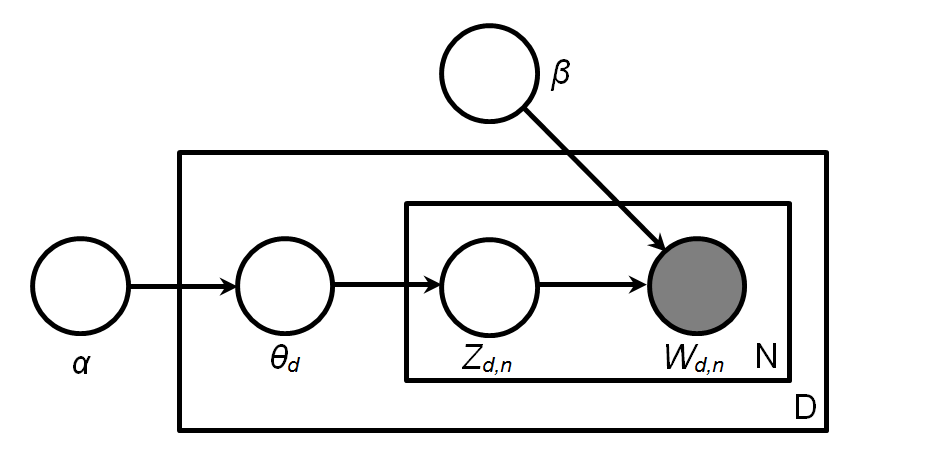
\includegraphics[scale=0.4]{images/lda-formal-model}

\caption{LDA topic model\textemdash{}unshaded nodes represent hidden variables; the remaining (shaded) node represents the words in each document
as the only observable variable. {\scriptsize Adapted from: \protect\href{http://en.wikipedia.org/wiki/Latent_Dirichlet_allocation}{http://en.wikipedia.org/wiki/Latent\_{}Dirichlet\_{}allocation}}}
\label{lda-formal-definition}

\end{figure}

In this graphical model:

\begin{itemize}
\item $\beta$ represents the $K$ topics that run through a collection of $D$ documents. 
\item Each $\beta_{k}$ is a distribution over the corpus vocabulary. 
\item The per-document topic distribution is parametrized by $\alpha$ ($\theta~Dir(\alpha)$) \footnote{$Dir(\alpha)$: Dirichlet distribution parametrized by $\alpha$.
}.
\item $\theta_{d}$ represents the topic distribution of the $d$-th document, being $\theta_{d,k}$ : proportion of topic $k$ on $d$.
\item $Z_{d,n}$ represents the topic assignment for the $n$-th term in document $d$ ($d$ contains $N$ terms). 
\item $W_{d}$ is the set of terms included in document $d$, being $W_{d,n}$: the $n$-th word in $d$. 
\end{itemize}

As stated before, the only observable variable in the LDA topic model is the collection of documents, namely $W$. Other variables ($\beta$, $\theta$, $Z$), are inferred by analyzing the joint distribution of the LDA generative process, defined as:

\begin{equation}
p(\beta_{1:K},\theta_{1:D},Z_{1:D},W_{1:D})=\prod_{i=1}^{K}p(\beta_{i})\prod_{d=1}^{D}p(\theta_{d})(\prod_{n=1}^{N}p(Z_{d,n}\mid\theta_{d})p(W_{d,n}\mid\beta_{1:K},Z_{d,n}))\label{eq:1}
\end{equation}

From the joint distribution in Eq. (\ref{eq:1}), it is derived the conditional distribution of $\beta$, $\theta$, $Z$ given $W$ (posterior distribution):

\begin{equation}
p(\beta_{1:K},\theta_{1:D},Z_{1:D}\mid W_{1:D})=\frac{p(\beta_{1:K},\theta_{1:D},Z_{1:D},W_{1:D})}{p(W_{1:D})}\label{eq:2}
\end{equation}

In the previous expression, the denominator $p(W_{1:D})$ is the marginal distribution of the observations, that is to say, the probability of observe the document collection under any thematic structure. Given that the number of possible thematic structures is exponentially large \cite{Blei:2003}, such a marginal distribution is intractable to estimate, so the posterior distribution in Eq. \ref{eq:2} can only be computed through approximation algorithms.

In general terms those algorithms fall into two categories: Sampling-based algorithms (e.g.: Gibbs sampling \cite{Geman:1984}) and Variational Bayesian methods, these latter usually being more effective than its sampling-based counterpart, while offering comparable precision. Variational methods posit a parametrized family of distributions over the structure of hidden variables of the model and subsequently deduce the closest member of such family to the posterior distribution in Eq. \ref{eq:2}, by using the \emph{Kullback-Leibler} divergence measure \cite{Shlens:2007}.
This way, the posterior estimation which was originally an inference problem, becomes now an optimization problem. 


\subsubsection{Application of LDA over information extracted from services documentation}
\label{subsub:Application-of-LDA}

The previous section addressed a study of the LDA topic model, which allow to define the hidden topics that run through a collection of documents. Topics in LDA may be devised as categories  that comprises semantically-related elements. This categorization, as opposed to traditional clustering techniques (like \emph{K-means}) is non-exclusive since a document from the collection may belong to multiple categories\footnote{Theoretically, all documents belong to all categories but, only few categories have a meaningful proportion of each document content.}. This way, LDA enables to expose useful relations within the collection not only at the document level but at the topic level too. 

The approach documented herein, comprises the application of the LDA model on the information extracted from the Web services documentation (according to the process outlined in section \ref{subsec:analysis-ws-doc}), for automatically categorizing and annotating it. Given that the service documentation focuses on describing the service operations (for SOAP and XML-RPC services) and services resources (for REST services), it was decided to generate a document for each operation/resource, containing the information related to it, that is, the categorization is performed at the operation/resource level.

Additionally, this approach proposes that categorization should be performed incrementally, so that the derived structure of categories gets updated as new documents (service operations/resources) become available, operating in an \emph{online learning} setting. However, the traditional LDA model doesn't support this online setting, so it was necessary to use an online variant of this model proposed by Hoffman et al. \cite{Hoffman:2010}, which uses a variational Bayesian algorithm to estimate the posterior distribution in Eq. \ref{eq:2}, from a stream of documents handled in small-sized batches. The authors of this online LDA variant evaluated the performance of their algorithm on a set of 3.3 million of randomly chosen articles from Wikipedia, and they proved that it is more precise and faster than the traditional LDA model.

In section \ref{sec:experimentation} we describe a prototype developed based on out proposal, which uses the online LDA algorithm for categorizing the documentation of a corpus of 200 real service descriptors extracted from the research dataset collected by Zhang et al. \cite{Zhang:2010} available at \href{http://www.wsdream.net/dataset.html}{http://www.wsdream.net/dataset.html}. 

\subsection{\emph{KNOWEB-S}: an RDF taxonomy for representing the derived service categorization}
\label{subsec:KNOWEB-S-RDF}

The third of the processes that shape the solution proposed in this approach, involves the construction of a taxonomy that formally encodes and represents the category structure generated by applying online LDA on Web services documentation. This taxonomy has been called \emph{KNOWEB-S} (\emph{KNOwledge representation for Web Services}). For specifying KNOWEB-S it was decided to use the data model that RDF embodies \cite{W3C:2004}, given the reasons listed below:

\begin{itemize}
\item \emph{Simplicity}: RDF allows to describe resources as statements in the form (\emph{subject}, \emph{predicate}, \emph{object}) or (\emph{resource}, \emph{property}, \emph{value}) called \emph{triples}.
\item \emph{Expressivity}: RDF offers an extensible language that allows to define classes and properties for specifying taxonomies and simple ontologies.
\item \emph{Standardization}: RDF is one of the so-called Semantic Web Standards, also being part of the recommendations from the \emph{World Wide Web Consortium} (W3C).
\item \emph{Wide adoption}: the RDF data model has been widely accepted by the scientific community and recognized by the industry for enabling integration and interoperability among services and applications. 
\end{itemize}

Additionally, RDF features SPARQL \cite{W3C:2008} as a query language for manipulating the information stored as RDF triples. Like RDF, SPARQL is also a W3C standard, recognized as one of the key technologies of the semantic Web.

This way, RDF provides for KNOWEB-S: a formal representation in a machine readable format; storage as a set of RDF triples (RDF graph); and a query language for searching and manipulating the information encoded in the taxonomy.
The section below describes the specific data model of KNOWEB-S, designed to represent the entities and relations that shape the taxonomy.

\subsubsection{KNOWEB-S Data Model}
\label{subsub:KNOWEBS-data-model}

The KNOWEB-S taxonomy arranges a set of categories which cluster semantically related documents (Web services operations or resources). Those categories are in turn defined as a sequence of representative terms. According to this definition, the entities and relations that make up the taxonomy are:

\begin{itemize}
\item Entities: 
\begin{itemize}
\item \emph{Document}: consists of information regarding a Web service operation or resource. 
\item \emph{Category}: groups related documents. 
\item \emph{Term}: defines a semantic unit associated to a particular category.
\end{itemize}

\item Relations: 
\begin{itemize}
\item \emph{Is member of}: between \emph{Document} and \emph{Category}. 
\item \emph{Has term}: between \emph{Category} and \emph{Term}
\end{itemize}
\end{itemize}

According to the LDA model used to perform the categorization, a document may belong to multiple categories depending on its per-category proportions.
This way the ``\emph{is member of}'' relation has a many-to-many (N:M) cardinality, and is weighted by the proportions of categories in each one of the documents, turning this into a non binary relation.

In the same way, the ``\emph{has term}'' relation between categories and terms is non binary---since it is weighted by the probability value that estimates the importance of the term to the category---and also has many-to-many cardinality.

Given these constraints, Figure \ref{data-model-KNOWEBS} shows the entity-relationship diagram for KNOWEB-S:

\begin{figure}
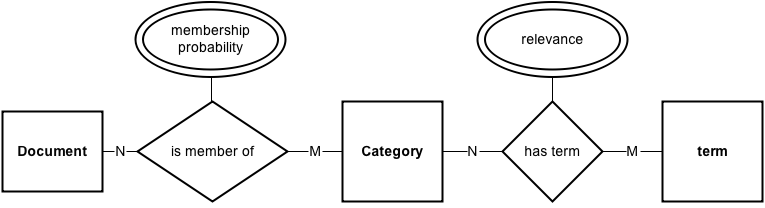
\includegraphics[scale=0.43]{images/KNOWEB-S-ER-en}

\caption{Entity-Relationship diagram of KNOWEB-S.}
\label{data-model-KNOWEBS}

\end{figure}

The previous diagram may be interpreted as follows: \textquotedblleft{}\emph{Documents} \emph{are members of} multiple \emph{Categories}, with certain \emph{membership probability}. In turn, \emph{Categories} \emph{has} multiple \emph{terms}, each one of them with a certain \emph{relevance}\textquotedblright{}. 

Next section details how to specify the KNOWEB-S data model in RDF. 

\subsubsection{RDF specification of KNOWEB-S}
\label{subsub:RDF-spec-of-KNOWEB}

As stated at the beginning of section \ref{subsec:KNOWEB-S-RDF}, RDF allows specifying taxonomies and simple ontologies, also known as vocabularies. To achieve this, an RDF-based standard language called RDFS (\emph{RDF Schema}) \cite{W3C:2004b} is employed. RDFS defines a set of artifacts through which it is possible to specify classes and their associated properties.

That way, in specifying the KNOWEB-S data model in RDFS, the \emph{entities} identified in the previous section are regarded as \emph{classes} and \emph{relations} turn into \emph{properties}. 

RDFS properties are binary relations, i.e. those that link two entities or an entity and a value. As mentioned earlier, relations of the KNOWEB-S data model are non-binary, since they link two individuals, with each link having an associated score (probability) that quantifies the relation. Therefore, there is no direct mapping of the identified relations (\textquotedblleft{}\emph{is member of}\textquotedblright{} and \textquotedblleft{}\emph{has term}\textquotedblright{}) into RDFS properties. According to recommendations of the W3C \cite{W3C:2006} regarding \emph{n-ary relations }definition in RDF, in cases like this, relations should be regarded as classes whose properties provide binary links for each attribute of the relation.

Thus, it is necessary to define two new entities and four new relations:

\begin{itemize}

\item New entities: 
\begin{itemize}
\item \emph{Membership relation}: defines a link between one Document and one Category while specifying the probability associated to it. 
\item \emph{Term relation}: defines a link between one Category and one Term while specifying the relevance of the term to the category.
\end{itemize}

\item New relations: 
\begin{itemize}
\item \emph{Category value}: between \emph{Membership relation} and \emph{Category} 
\item \emph{Membership probability}: between \emph{Membership relation} and a numerical value. 
\item \emph{Term value}: between \emph{Term relation} and Term. 
\item \emph{Term probability}: between \emph{Term relation} and a numerical
value.
\end{itemize}
\end{itemize}

Figure \ref{KNOWEBS-data-model-RDF} illustrates the entity-relationship diagram of KNOWEB-S, which includes these new entities and relations:

\begin{figure}
\center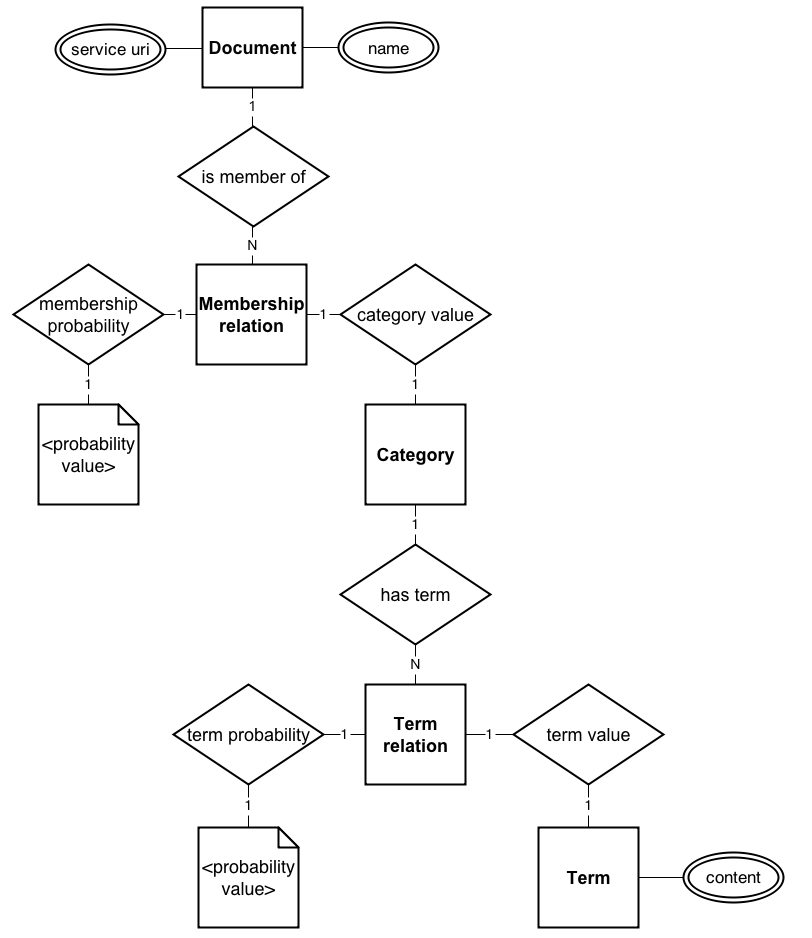
\includegraphics[scale=0.48]{images/KNOWEB-S-RDF-en}

\caption{Entity-relationship diagram of KNOWEB-S adapted to RDFS.}
\label{KNOWEBS-data-model-RDF}
\end{figure}


Finally, listing \ref{lis:KW-RDF-Specification} shows the KNOWEB-S data model, using the RDFS XML syntax for specifying it. 

\begin{scriptsize}
\begin{lstlisting}[caption={RDF Specification of KNOWEB-S},label={lis:KW-RDF-Specification}]

<?xml version="1.0" encoding="UTF-8" ?> 
<rdf:RDF
	xmlns="http://www.topicalizer.org/web_api_model.rdf#"
	xmlns:rdf="http://www.w3.org/1999/02/22-rdf-syntax-ns#"
	xmlns:rdfs="http://www.w3.org/2000/01/rdf-schema#"
	xml:base="http://www.topicalizer.org/web_api_model.rdf">   
<rdfs:Class rdf:ID="Category"/>
<rdfs:Class rdf:ID="Operation"/>
<rdfs:Class rdf:ID="Membership_Relation"/>
<rdfs:Class rdf:ID="Term"/>
<rdfs:Class rdf:ID="Term_Relation"/>
<rdf:Property rdf:ID="is_member_of">
	<rdfs:domain rdf:resource="#Operation"/>
	<rdfs:range rdf:resource="#Membership_Relation"/>
</rdf:Property>
<rdf:Property rdf:ID="category_value">
	<rdfs:range rdf:resource="#Category"/>
	<rdfs:subPropertyOf 
rdf:resource="http://www.w3.org/1999/02/22-rdf-syntax-ns#value"/>
	<rdfs:domain rdf:resource="#Membership_Relation"/>
</rdf:Property>
<rdf:Property rdf:ID="membership_probability">
	<rdfs:range 
	    rdf:resource="http://www.w3.org/2001/XMLSchema#double"/>
	<rdfs:domain rdf:resource="#Membership_Relation"/>
</rdf:Property>
<rdf:Property rdf:ID="has_term">
	<rdfs:domain rdf:resource="#Category"/>
	<rdfs:range rdf:resource="#Term_Relation"/>
</rdf:Property>
<rdf:Property rdf:ID="term_value">
	<rdfs:range rdf:resource="#Term"/>
	<rdfs:subPropertyOf 
rdf:resource="http://www.w3.org/1999/02/22-rdf-syntax-ns#value"/>
	<rdfs:domain rdf:resource="#Term_Relation"/>
</rdf:Property>
<rdf:Property rdf:ID="term_probability">
	<rdfs:range 
	    rdf:resource="http://www.w3.org/2001/XMLSchema#double"/>
	<rdfs:domain rdf:resource="#Term_Relation"/>
</rdf:Property>
<rdf:Property rdf:ID="has_content">
	<rdfs:range 
	    rdf:resource="http://www.w3.org/2001/XMLSchema#string"/>
	<rdfs:domain rdf:resource="#Term"/>
</rdf:Property>
<rdf:Property rdf:ID="has_name">
	<rdfs:range 
	    rdf:resource="http://www.w3.org/2001/XMLSchema#string"/>
	<rdfs:domain rdf:resource="#Operation"/>
</rdf:Property>
<rdf:Property rdf:ID="has_service_uri">
	<rdfs:range 
	    rdf:resource="http://www.w3.org/2001/XMLSchema#anyURI"/>
	<rdfs:domain rdf:resource="#Operation"/>
</rdf:Property>
</rdf:RDF> 
\end{lstlisting}
\end{scriptsize}